\documentclass[a4paper,11pt]{book}
\usepackage[top=3.5cm, bottom=3.5cm, left=3.5cm, right=3.5cm]{geometry}\usepackage[T1]{fontenc}
\usepackage[utf8]{inputenc}
\usepackage[english]{babel}
\usepackage{lmodern}
\usepackage{amsmath}
\usepackage{amsfonts}
\usepackage{amssymb}
\usepackage{amsthm}
\usepackage{graphicx}
\usepackage{color}
\usepackage{xcolor}
\usepackage{url}
\usepackage{theorem}
\usepackage{textcomp}
\usepackage{listings}
\usepackage{hyperref}
\usepackage{parskip}
\usepackage{tikz}
\usepackage{float}
\usepackage{fancybox}
\usepackage{fancyhdr}

\pagestyle{fancy}
\fancyhf{}
\fancyhead[LE,RO]{\thepage}
\fancyhead[RE]{\leftmark}
\fancyhead[LO]{\rightmark}

\renewcommand{\chaptermark}[1]{\markboth{Chapter \thechapter: #1}{}}

\graphicspath{{Sketches/}}


\newcommand{\doctitle}{Fluid Mechanics}
\newcommand{\docauthor}{Course of Tobias Schneider\\Trancription by Tim Tschanz}

\title{\doctitle}
\author{\docauthor}
\date{\today}

\hypersetup{
    pdftitle={\doctitle},
    pdfauthor={\docauthor},
}

\setlength{\headheight}{13.6pt}


\begin{document}
\begin{titlepage}
    \centering
    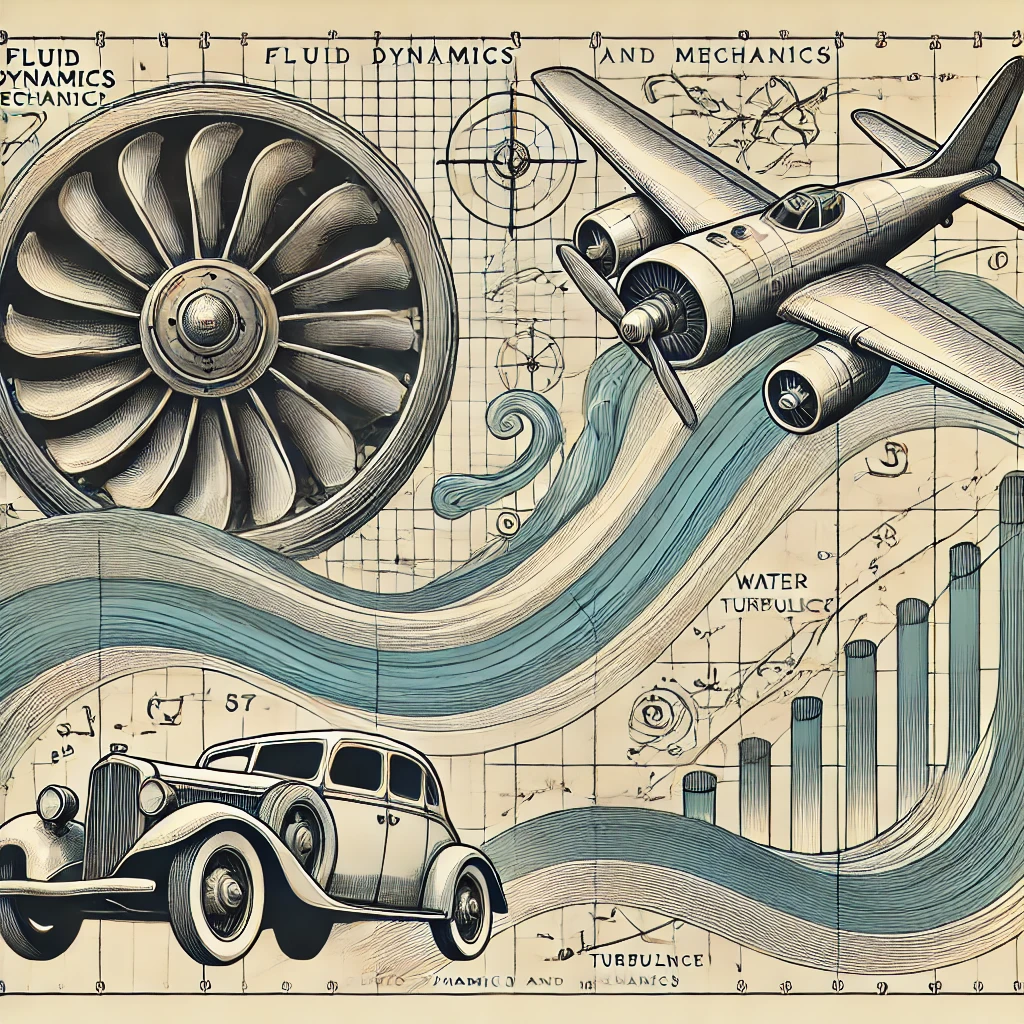
\includegraphics[width=\textwidth]{Cover_Image.png}
    {\huge\bfseries \doctitle\par}
    {
        \vspace{1cm}
        {\large \docauthor\par}
        \vspace{1cm}
    }
    {\large \today\par}
\end{titlepage}

\tableofcontents

\chapter{Introduction}

This chapter is based on Munson Chapter 1.
\section{Definitions}
\subsection{Fluid}
A fluid is a substance that \textbf{deforms continuously} under any \textbf{shear stress}\footnote{A shear stress $\tau$ is the tangential component of a force that acts on an surface}. Equivalently we can say: A fluid is a material that cannot statically resist a shear stress. It needs to move in order to resist a shear stress.

The resistance of a fluid to shear stress is determined by viscosity

\subsection{Basic Laws of Physics}
The basic laws of physics that a fluid dynamics problem must satisfy are:
\begin{enumerate}
    \item conservation of mass
    \item Newton's 2nd law  ("conservation of momentum")
    \item conservation of energy (first law of thermodynamics)
    \item 2nd law of thermodynamics
\end{enumerate}

\subsection{Properties of a fluid}
\begin{itemize}
    \item \textbf{density} $\rho=\frac mV,\qquad [\rho]=\frac {\operatorname{kg}}{\operatorname{m}^3}$
    \item \textbf{specific volume} $v=\frac Vm=\rho^{-1}\qquad [v]  =\frac {\operatorname{m}^3}{\operatorname{kg}}$
    \item \textbf{specific weight} $\gamma=\rho g\qquad [\gamma]=\frac{\operatorname{kg}\operatorname{m}}{\operatorname{m}^3\operatorname{s}^2}=\frac{\operatorname{N}}{\operatorname{m}^3}$
    \item \textbf{specific gravity} $SG=\frac{\rho}{\rho_{H_2O}}$
\end{itemize}
\subsection{Normal Conditions}
% Context?
% From Thermodynamics: $rho = f(T,p)$\footnote{This is only applicable if we are not in a two-phase region.}
Normal conditions are at athmospheric pressure ($1atm$) at $300K$. At these conditions:
\begin{itemize}
    \item $\rho_{H_2O} = 1000 \mathrm{kg/m^3}$
    \item $\rho_{Air} = 1.22 \mathrm{kg/m^3} \approx \frac{\rho_{H_2O}}{1000}$
\end{itemize}

\subsection{Ideal Gas Law}
$$
\rho = \frac{p}{RT}
$$
where $p$ is the \textbf{absolute pressure} (pressure relative to vacuume), $T$ is the \textbf{absolute temperature} (in $\mathrm{K}$), $\rho$ is the \textbf{density} and $R$ is the \textbf{specific gas constant} (sometimes denoted as $R_s$).

\subsection{Viscosity}
To quantify the response of a fluid to a shear stress, we need to have a measure of how quickly a fluid moves.

\subsubsection{No Slip Condition, Shear Strain Rate}
\begin{center}
\shadowbox{At a solid boundary a fluid will have zero velocity relative to the boundary.}
\end{center}
\begin{figure}[H]
    \begin{center}
    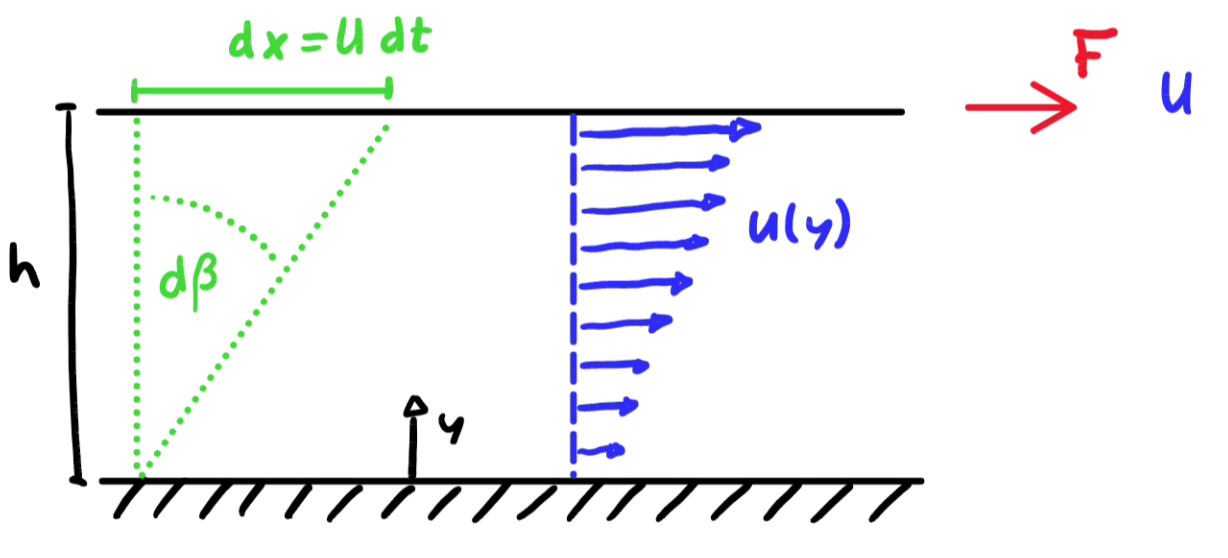
\includegraphics[width=0.4\textwidth]{NoSlip.png}
    \caption{Two plates have a fluid in between. After applying a pure shear force, the top plate moves with velocity $U$. This moves our magically marked atoms on the top by $dx=Udt$.}
    \end{center}
\end{figure}
We can pose the tangent of $d\beta$ to find the deplacement at a height $h$. For small deplacements we can find the change in angle over time to be the \textbf{shear strain rate} $\dot \gamma$
$$
\tan d\beta = \frac {dx}h \approx d\beta \qquad d\beta << 1\implies \frac {d\beta}{dt} = \frac{dx}{hdt}=\frac Uh =: \dot \gamma\qquad [\dot \gamma] = s^{-1}
$$
\paragraph{Notes}
Anywhere in the domain, we can approximate that
$$
\frac Uh \approx\frac {dU}{dy}
$$
\subsection{Newtonian Fluids}
How can we relate the equations of shear stress and shear strain rate? 
We define as \textbf{newtonian fluids} as all the fluids, where the relationship between the applied shear stress is proportional to the shear strain rate (i.e. how much does it respond):
\begin{equation}
\tau = \frac FA \propto \frac {dU}{dy}\implies \tau = \mu \frac{dU}{dy}\label{eq:newtonian_fl}
\end{equation}

\shadowbox{For a newtonian fluid, the more force I apply, the faster it moves (linearly).}
\subsection{Viscosity}

\subsubsection{Dynamic Viscosity}
We define the factor of linearity $\mu$ in \ref{eq:newtonian_fl} to be \textbf{viscosity} (often called dynamic viscosity)
$$
[\mu] = \frac {\mathrm{kg}}{\mathrm m\cdot \mathrm s}
$$

\subsubsection{Kinematic Viscosity}

$$
\nu := \frac \mu \rho\qquad [\nu] =\frac {\mathrm m^2}{s} 
$$
\subsubsection{Notes} 
\begin{itemize}
    \item The stress-strain rate relation in general can be more complex in other flow geometries. But for newtonian fluids it remains linear.
    \item In theory, viscosity $\mu$ is tensor of rank 4. Through symetries, this often collapses to a scalar.
    \item In solids, there are so called Hookean materials which are analogous to Newtonian fluids, where the strain is linear whereas in newtonians the strain rate is linear.
\end{itemize}
\subsubsection{Common Values of Viscosity}
At normal conditions:
\begin{figure}[H]
    \begin{minipage}{0.45\textwidth}
        \centering
        \begin{tabular}{ll}
        \textbf{Material} & \textbf{Viscosity $\mu$ in $\mathrm{kg}/(\mathrm m\cdot \mathrm s)$}\\
        \hline
        Air      & $1.8\cdot 10^{-5}$                         \\
        \hline
        Water    & $1.1\cdot 10^{-3}$                          \\
        \hline
        "Oil"    & $0.4$                       
        \end{tabular}

    \end{minipage}
    \hfill
    \begin{minipage}{0.45\textwidth}
        \centering
        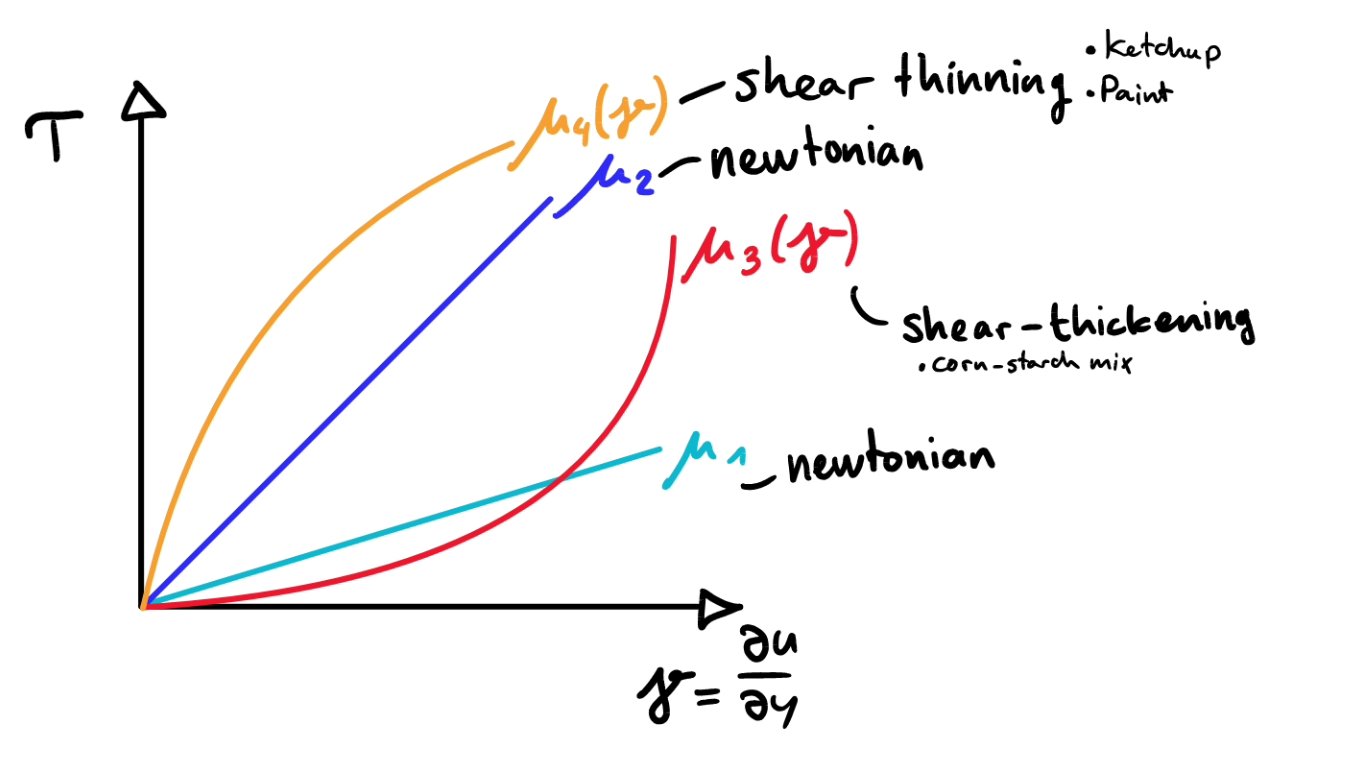
\includegraphics[width=\textwidth]{Newtonian_NonNewtonian.png}

    \end{minipage}
\end{figure}

\paragraph{cgs: Poise}
The poise (only centi-poise is really used) is a commonly used unit for viscosity
$$
\frac{\mathrm g}{\mathrm{cm}\cdot\mathrm s} =: \mathrm{poise} = \mathrm p = 100 \mathrm{cp}
$$

\section{Application: Simple Flow Problem (Munson 1.69)}
We consider the setup in the figure bellow. Two fluids are seperated by an infinite plate at a given height. The top most plate moves at a given velocity $U$. We want to determine the velocity $V$ of the center plate. Additionally we assume that $\mu_2=2\mu_1$.

\begin{figure}[H]
    \begin{minipage}{0.45\textwidth}   
                \centering
            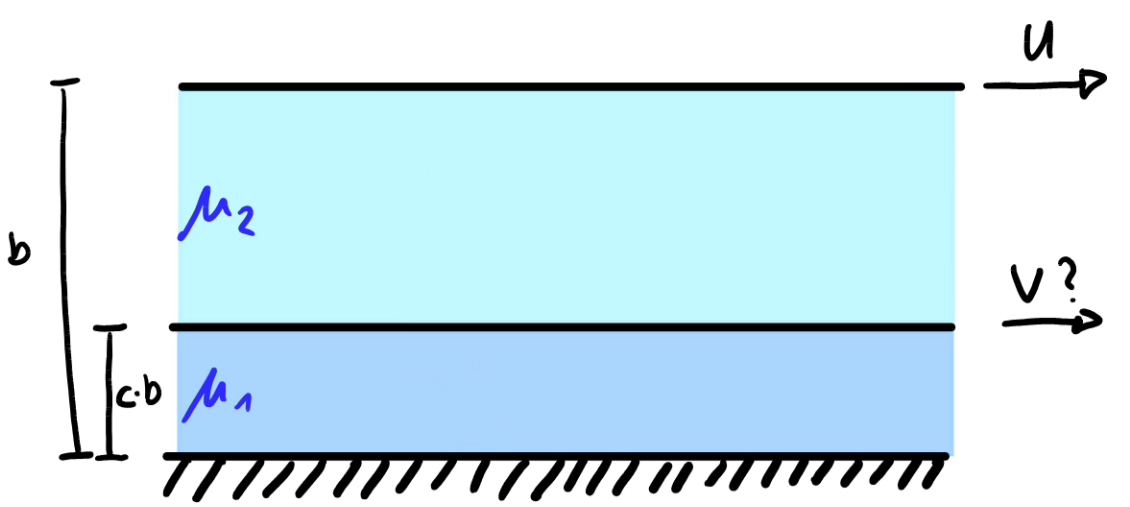
\includegraphics[width=\textwidth]{FlowProblem_1_69a.png}
            \caption{The two fluids with their respective viscosities. The ground plate is fixed and the top moves at a given velocity.}            
    \end{minipage}
    \hfill
    \begin{minipage}{0.45\textwidth}
        \centering
        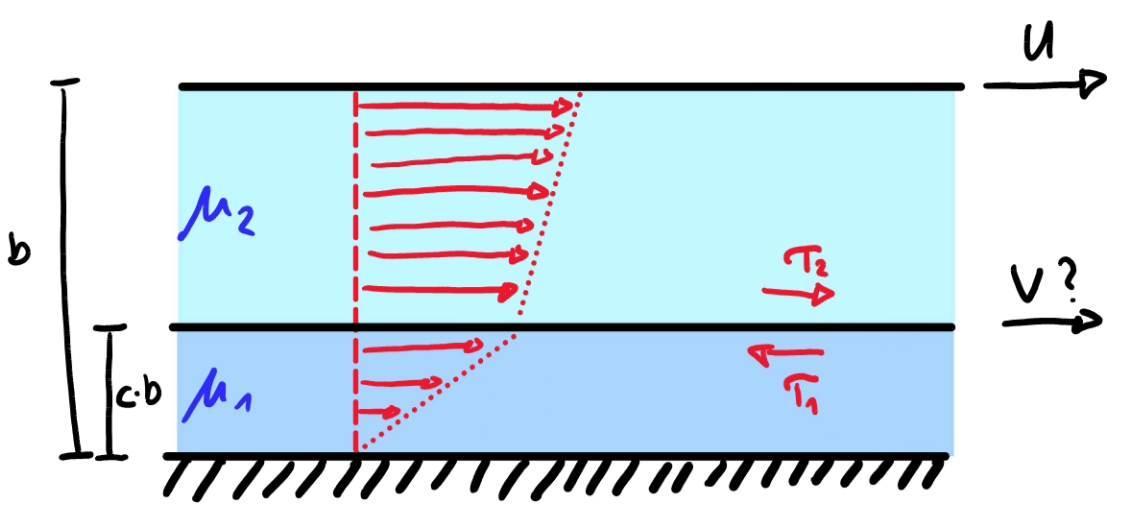
\includegraphics[width=\textwidth]{FlowProblem_1_69b.png}
        \caption{We add shear stresses to the drawing and draw the displacement distribution along the height.}
    \end{minipage}
\end{figure}

We apply the force balance on the middle plate:
\begin{equation*}
    \begin{split}
    \sum F_H = \tau_2A-\tau_1A &\stackrel{*}{=} 0\qquad *: a= 0\\
    \implies \tau_1 &= \tau_2
    \end{split}
\end{equation*}
Expressing $\tau_1$ in terms of variables yields:
$$
\tau_1 = \mu_1\frac V{cb}\stackrel{!}{=}\tau_2=\mu_2\frac{U-V}{(1-c)b}
$$
After solving for $V$ to get:
$$
V=\frac {2c}{1+c}U
$$
To verify boundary conditions, we test for $c=0$ and $c=1$:
$$
\begin{cases}
c=0\implies V=0\\
c=1 \implies V = U
\end{cases}
$$
These results make sense to us.
\chapter{Hydrostatics}
This chapter is based on Munson Chapter 2.

\section{Pressure at a point}
\label{sec:pressure_at_point}
We commonly assume that pressure at a point is a scalar. However, pressure is the component of stress which is normal to a surface.

We consider a wedge-shaped element of fluid. We apply Newton's force balance to the element, for this we need to transform the pressures acting on the surfaces into forces $F_y,F_z,F_s$. Furthermore, we make the assumption that there are no tangential forces on any of the surfaces: we are neglecting all shearing forces.


\begin{figure}[H]
	\centering
	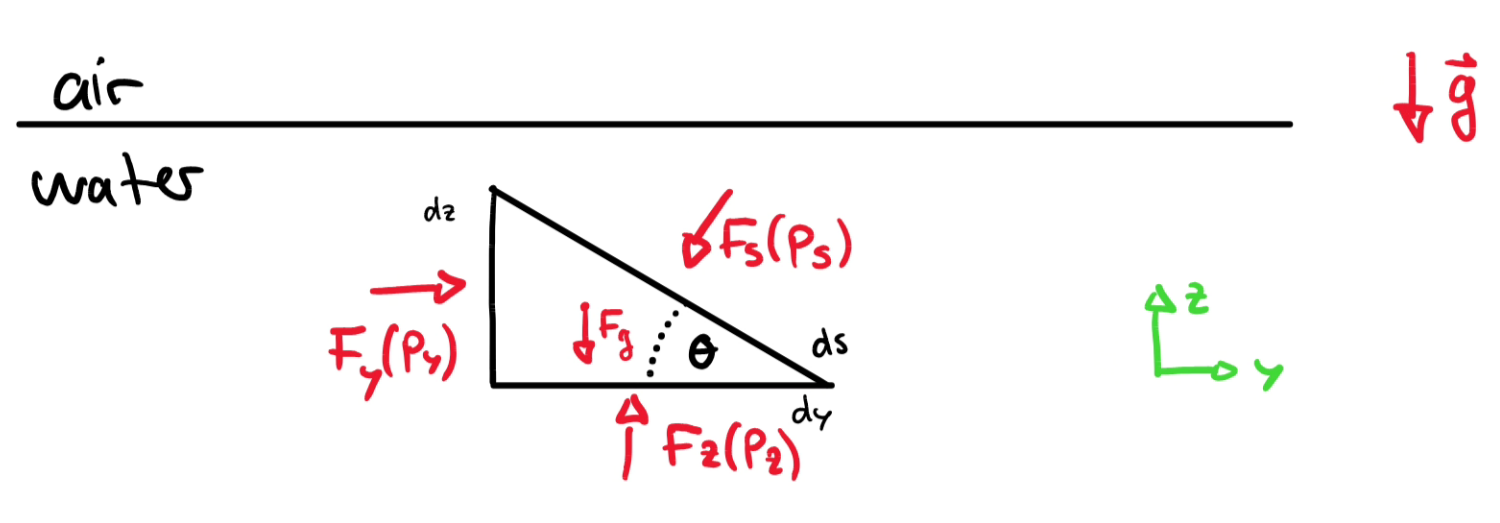
\includegraphics[width=0.6\textwidth]{WedgeElement.png}
	%\caption{}            
\end{figure}

Newton's second law in $z$ direction yields:
\begin{equation*}
	\begin{split}
		\sum \vec F &= m \vec a \\
		\quad F_z = p_z\cdot dx\cdot dy - p_s \cdot ds\cdot dx\cdot \cos \theta-\rho g dV &= \rho dV a_z\qquad \left | \begin{cases}ds = \frac {dy} {\cos\theta}\\ dV = \frac{dz\cdot dy}{2}dx\end{cases}\right.\\
		p_z-p_s -\rho g \frac{dz}2 &= \rho \frac {dz}2a_z\\
		dx,dy,dz\to 0 \implies p_z&=p_s
	\end{split}
\end{equation*}
Similarly we can do the calculation in $x$ and $y$, which results in a final result of
$$
p_z=p_x=p_y=p_s
$$
for any angle $\theta$.

Seeing that the pressure is equal for any direction, we can conclude that $p$ is a scalar
\section{Equation for Pressure Field}
Using the same idea as for \ref{sec:pressure_at_point}, we look at a box.
\begin{figure}[H]
	\centering
	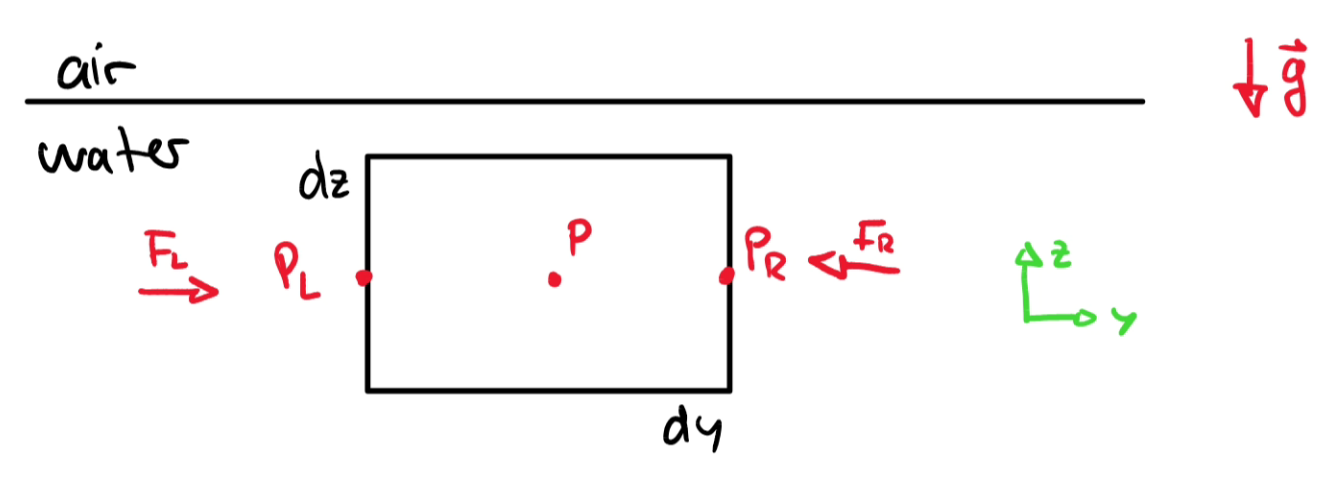
\includegraphics[width=0.6\textwidth]{CubeElement.png}
	%\caption{}            
\end{figure}
We use Taylor expansion to express $p_l$ and $p_r$:
\begin{equation*}
	\begin{split}
		p_r &= p + \left.\frac{dy}{2}\frac{\partial p}{\partial y}\right|_0+\dots\\
		p_l &= p - \left.\frac{dy}{2}\frac{\partial p}{\partial y}\right|_0+\dots\\
		\implies F_R &= p_r\cdot dx\cdot dz = \left( p + \left. \frac{dy}{2}\frac{\partial p}{\partial y}\right|_0\right)dx\cdot dy+\dots\\
		\implies F_L &= p_l\cdot dx\cdot dz = \left( p - \left. \frac{dy}{2}\frac{\partial p}{\partial y}\right|_0\right)dx\cdot dy+\dots\\
	\end{split}
\end{equation*}
We apply force balance in $y$:
\begin{equation*}
	\begin{split}
		-F_R+F_L&=\rho dVa_y\\
		\left.-dy\frac{\partial p}{\partial y}\right|_0\cdot dx\cdot dz &= \rho\cdot dx\cdot dy\cdot dz\cdot a_y+\dots \\
		-\left.\frac{\partial p}{\partial y}\right|_0&=\rho a_y+\dots
		\stackrel{\lim_{dx,dy,dz\to 0 }}{\implies}\left.-\frac{\partial p}{\partial y}\right|_0=\rho a_y
	\end{split}
\end{equation*}
We could do the same calculation in the $x$ and $z$ direction, where the weight needs to be considered. We can rewrite Newtons second law per unit volume:
\begin{equation}
	\boxed{-\nabla p -\rho g\hat k =\rho \vec a}
	\label{eq:newtons_second_law_per_unit_volume}
\end{equation}
\paragraph{Remark} Remember that we neglected shear forces to derive this result. It is only valid if we have no shear forces.

\section{Fluids at Rest}
When a fluid is at rest, from newtons second law we can say that $\vec a = \vec 0$. The derived equation for newton seconds law per unit volume \eqref{eq:newtons_second_law_per_unit_volume} then yields:
\begin{equation}
	\begin{split}
		-\frac{\partial p}{\partial x} &= 0\\
		-\frac{\partial p}{\partial y} &= 0\\
		-\frac{\partial p}{\partial z}-\rho g &= 0
	\end{split}
	\label{eq:fluid_at_rest}
\end{equation}
Which means that the pressure only depends on $z$:
$$
p = p(z)
$$
We can solve the differential equation in \eqref{eq:fluid_at_rest} to find the pressure function explicitly:
\begin{equation}
	\begin{split}
		\frac{\partial p}{\partial z} &= -\rho g\\
		\int dp &= - \int \rho g dz\\
		\Delta p &\stackrel{(*)}{=} - g \int \rho\, dz
	\end{split}
	\label{eq:pressure_difference}
\end{equation}
Where at $(*)$ we assumed the gravitational acceleration to be constant.
\subsection{Incompressible Fluid}
If $\rho$ is constant, a fluid is considered to be an incompressible fluid. The equation for pressure difference \eqref{eq:pressure_difference} is simple to solve:
\begin{equation*}
	\Delta p = -g\rho \Delta z
\end{equation*}
Choosing a coordinate system that goes down with $h$ (height below reference surface) and has its origin such that $h_0=0$ at $p_0$ we can reorder
\begin{equation}
	\boxed{p(h)=\rho g h + p_h}
	\label{eq:pressure_incompressible}
\end{equation}
\paragraph{Remark}
Remember that $p$ is absolute pressure, relative to vacuum. Compared to gage pressure, which is relative to a reference pressure such as the atmospheric pressure. Gage pressure in the above equation \eqref{eq:pressure_incompressible} would be $p-p_h = \rho g h$

\subsection{Compressible Fluid}
To think of compressible fluids (i.e. $d\rho \ne 0$) such as ideal gases, we recall the ideal gas law: $p=\rho R T\implies \rho = p/{RT}$. Combining with the z component of \eqref{eq:fluid_at_rest} we know:
\begin{equation*}
	\begin{split}
		\frac{dp}{dz} &= -\frac{p}{RT}g\\
		\frac 1p \,dp &= -\frac g{RT} dz\qquad (\ast)\\
		\ln(p) &= -\frac g{RT}z + C\\
		p(z) &= C_1\exp\left(-\frac{g}{Rt}z\right)
	\end{split}
\end{equation*}
We assumed at $(\ast)$ that we are at an isothermal atmosphere ($T=const$). To find the integration constant, we pose that at $z=0$ we have a pressure of $p_0$. This yields the \textbf{pressure of ideal gas for isothermal atmosphere}:
\begin{equation}
	\boxed{p(z)=p_0e^{-\frac g{RT}z }}
	\label{eq:pressure_compressible_isothermal}
\end{equation}

Instead of assuming an isothermal atmosphere, we can assume a linear regression of temperature as a function of height, which is accurate up to a certain height (see \ref{fig:temperatureatmosphere}).
\begin{figure}
	\centering
	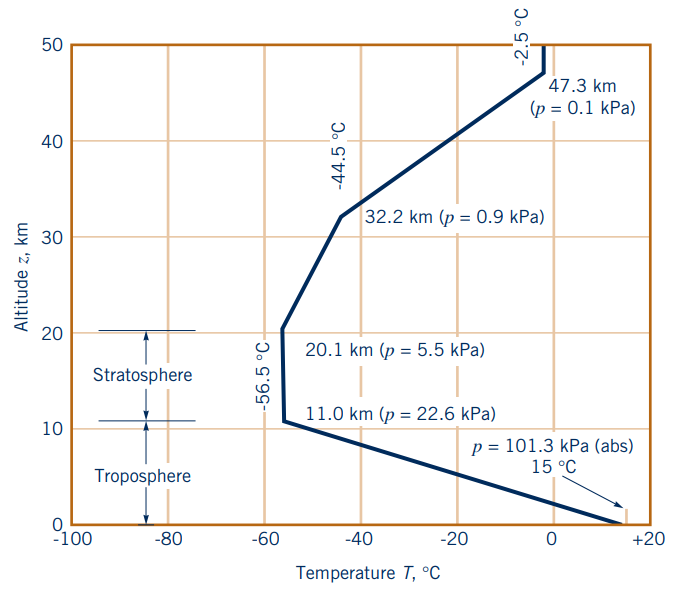
\includegraphics[width=0.4\linewidth]{Sketches/TemperatureAtmosphere}
	\caption{The temperature gradient in our atmosphere (Munson et al, Fluid Dynamics)}
	\label{fig:temperatureatmosphere}
\end{figure}
This leads us, with the \textbf{Standard Atmosphere} of $T(z) = T_0-\beta z$ to the following result of the \textbf{pressure of ideal gas for non-isothermal atmosphere}:
\begin{equation}
	\boxed{p(z)=p_0(1-\frac{\beta z}{T_0})^{\frac{g}{R\beta}}}
\end{equation}


\paragraph{Notes}
The units of pressure are Newton per square-meters, yielding Pascal. $1\ \mathrm{atm}$ is equivalent to $1.01\cdot 10^5\ \mathrm{Pa}$ and $760\ \mathrm{mmHg}$.

\section{Forces on Submerged Surfaces}

\subsection{Flat Surfaces}
\textit{(Munson 2.8)}\hfill\\

We consider a flat surface submerged in an incompressible fluid at an angle $\theta$. 
\begin{figure}[H]
	\centering
	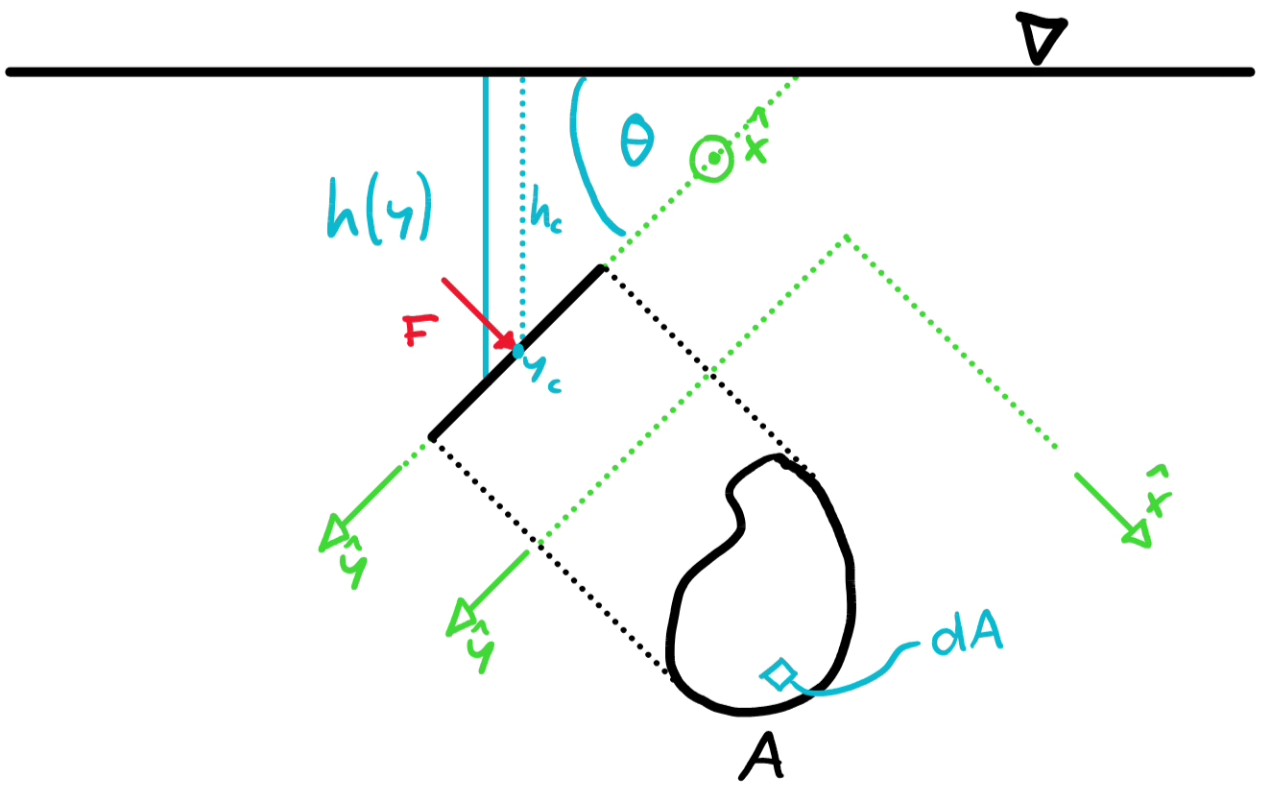
\includegraphics[width=0.5\linewidth]{Sketches/ForceOnFlatSurface}
	\caption{}
	\label{fig:forceonflatsurface}
\end{figure}

We can immediately say:
\begin{equation*}
	p = \rho gh, \qquad h = \sin\theta
\end{equation*}
We integrate over the surface:
\begin{equation*}
	\begin{split}
		F & =\int_A \rho gh \,dA\\
		&=\int_A \rho gy\sin\theta\, dA\\
		&=\rho g \sin\theta \int_A y\, dA\\
		&= \rho g \sin\theta A y_c\\
	\end{split}
\end{equation*}
We recognized the integral as the centroid\footnote{the "average" point, defined as $A^{-1}\int_A y\,dA$. Common values can be found in \ref{fig:geometricalpropertiesshapes}} multiplied by the area at $(\ast)$. Recognizing that $\sin\theta y_c = h_c$, and $\rho g h_c = p_c$. This yields
\begin{equation}
	\boxed{F=p_c A}
\end{equation}
Which makes intuitive sense: The magnitude of the resultant force is given by the pressure at the centroid times the area. It is independent of the orientation ($\theta$ in this case).

To find the point of application of the resultant, we want the distributed force to generate the same moment as the resultant force. We choose the origin of our coordinate system to calculate the moments:
\begin{figure}[H]
	\centering
	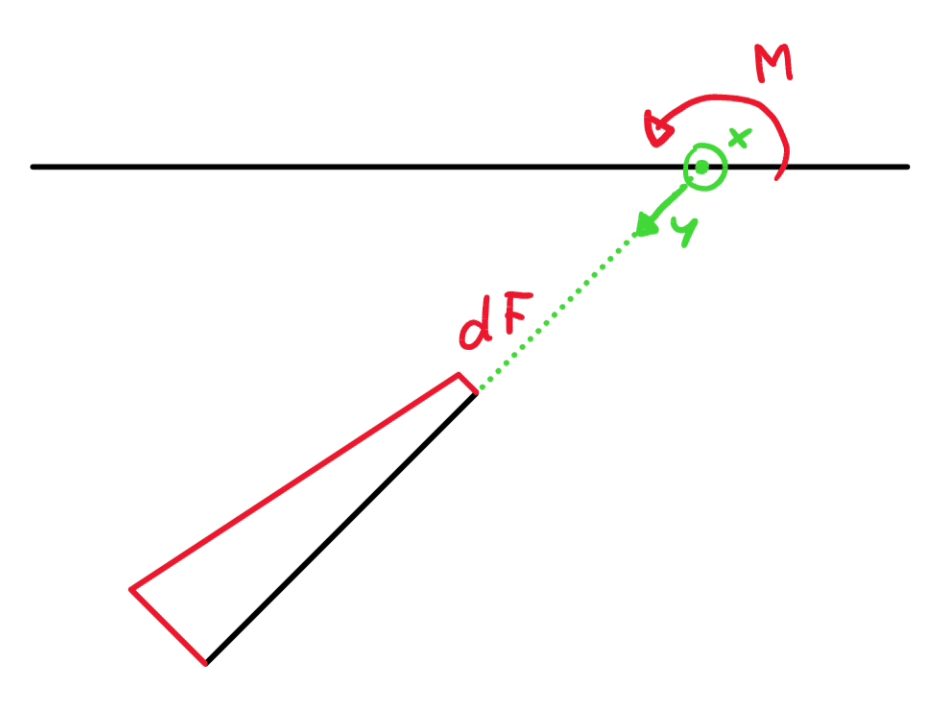
\includegraphics[width=0.5\linewidth]{Sketches/ForceOnFlatSurface_Moment}
	\caption{}
	\label{fig:forceonflatsurfacemoment}
\end{figure}

\begin{equation*}
	\begin{split}
	dF &= \rho gh\,dA = \rho g y\sin\theta dA\\ 
	dM &= y\,dF = \rho\sin\theta y^2\, dA\\
	 M &= \rho g\sin\theta \int_A y^2\, dA\\
	 &= \rho g\sin\theta I_x
	\end{split}
\end{equation*}
Using Steiner's Theorem ($I_x=I_{xc}+Ay_c^2$), we can translate the moment of inertia to the centroid axis and write the final condition for the point of application of the resultant force:
\begin{equation*}
	\begin{split}
		M &= \rho g \sin\theta (I_{xc}+Ay_c^2) = F y_r = \rho g y_c\sin\theta A y_r\\
		\implies &\boxed{y_r = y_c + \frac{I_{xc}}{y_c A }}
	\end{split}
\end{equation*}
From this equation, the application point is always bellow the centroid.


\begin{figure}[H]
	\centering
	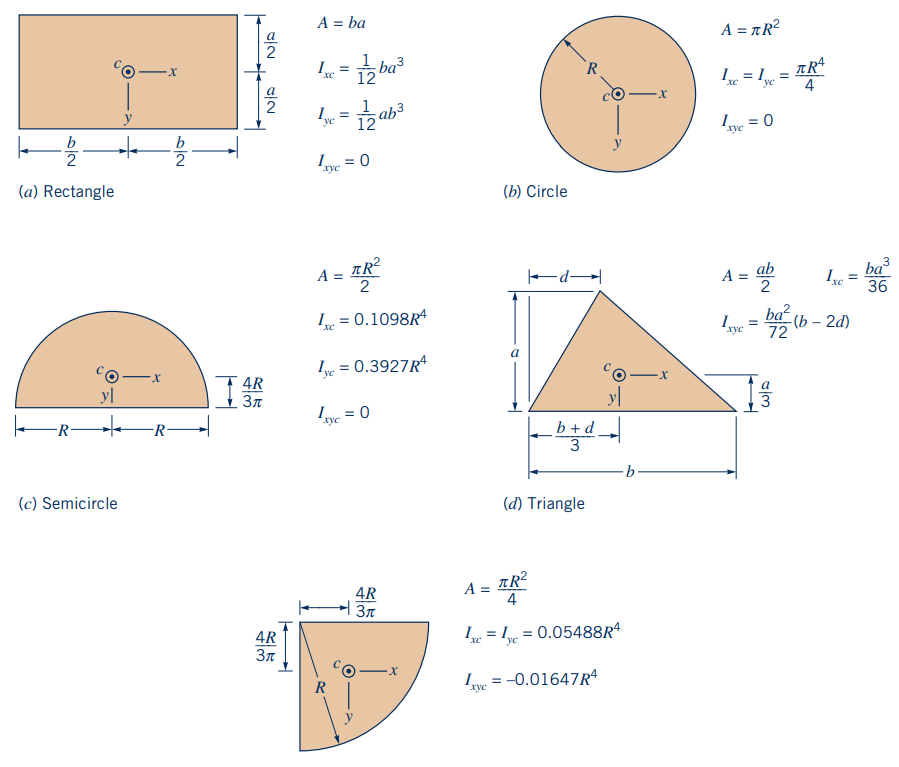
\includegraphics[width=0.7\linewidth]{Sketches/GeometricalPropertiesShapes}
	\caption{Geometrical properties of common shapes (Munson et al, Fluid Dynamics)}
	\label{fig:geometricalpropertiesshapes}
\end{figure}

\subsection{Curved Surfaces}
\textit{(Munson 2.10)}\hfill\\

We decompose the resultant force $\vec F_R$ into its components $\hat i, \hat j$. For both components we integrate over the area, approaching each infinitesimal area $dA$ as a flat surface.

\begin{equation*}
	\begin{split}
		\vec F_R &= F_H\hat i + F_V \hat j\\
		dF &= pdA
	\end{split}
\end{equation*}
Through geometry, we find that $F_H$ is the force acting on the vertical projection of the surface:
\begin{equation*}
	dF_H = pdA\cos\theta = pdA_V\implies F_H=\int pdA_V
\end{equation*}
\begin{figure}[H]
	\centering
	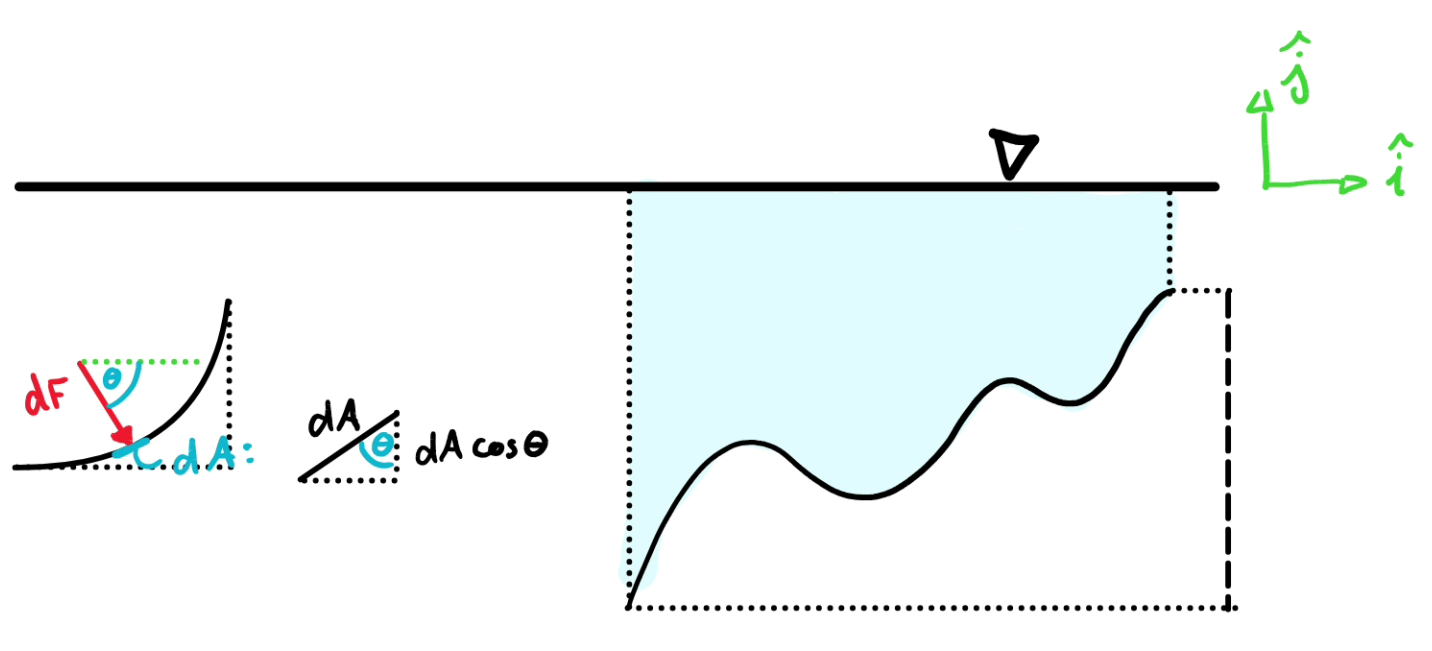
\includegraphics[width=0.7\linewidth]{Sketches/ForceOnCurvedSurface}
	\label{fig:forceoncurvedsurface}
\end{figure}

Similarly, we find that for the vertical component, the force acting vertically on the surface is equal to the weight of the water column above surface:
\begin{equation*}
	dF_V=pdA\sin\theta = \rho ghdA\sin\theta \rho g dV \implies F_V = \int_A g\rho dV 
\end{equation*}


\section{Example Problems}
\subsection{Force on a Tank Sidewall}
Consider a tank sidewall. What is the total resultant force on the surface of the sidewall?
\begin{figure}[H]
	\centering
	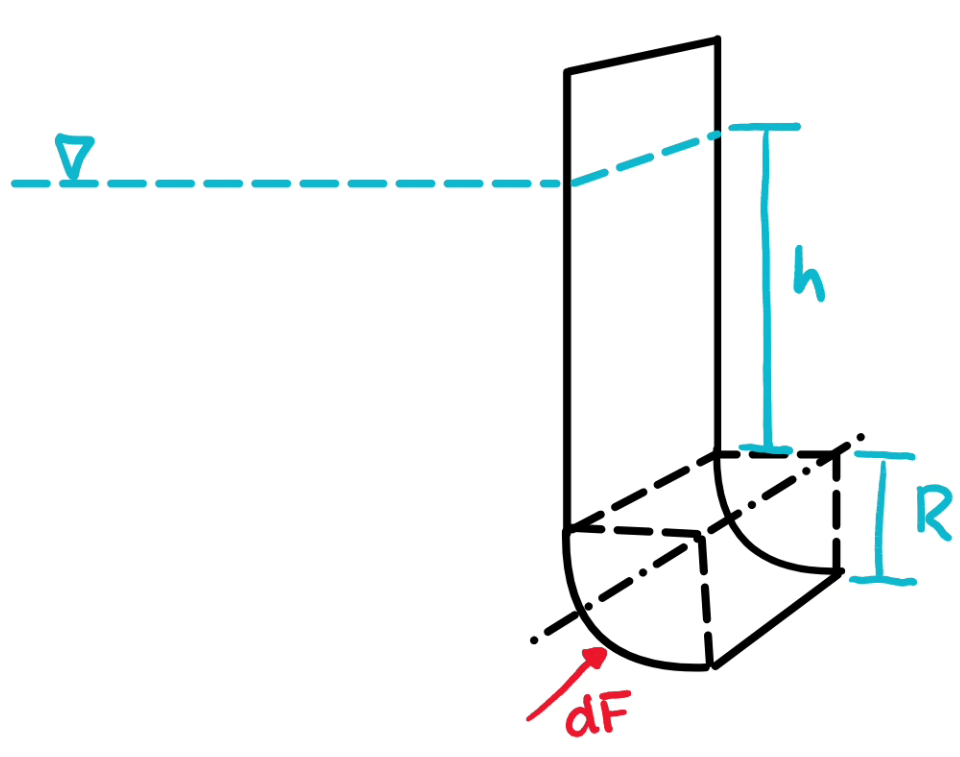
\includegraphics[width=0.4\linewidth]{Sketches/ExampleTankSidewall}
\end{figure}

The vertical component:
\begin{equation*}
	F_V = \int_AdF_V = \left[hRw+\frac{\pi R^2}{4}w\right] \rho g
\end{equation*}
horizontal:
\begin{equation*}
	\begin{split}
		F_H &= \int_A dF_H \\
		&=\text{force on vertical projection} \\
		&= \text{Area * pressure at centroid} \\
		&=  p_cA_V = \rho g\left(h+\frac R2 \right)R_w
	\end{split}
\end{equation*}


\subsection{Archimedes' Principle}
\begin{figure}[H]
	\centering
	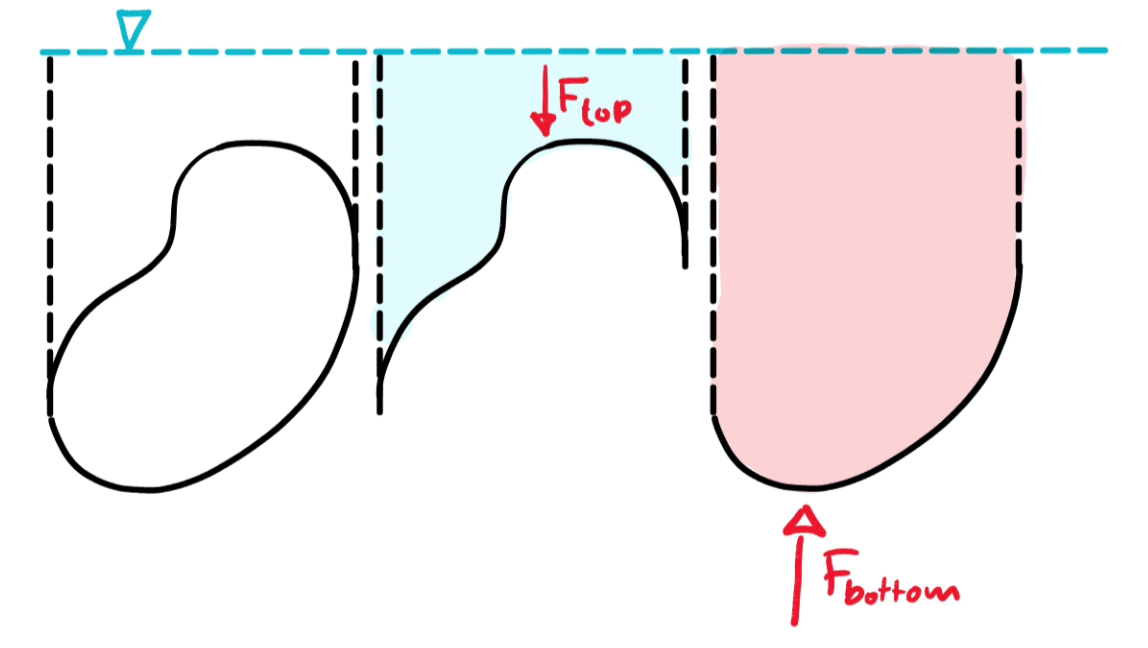
\includegraphics[width=0.7\linewidth]{Sketches/Archimedes}
	\label{fig:archimedes}
\end{figure}
$$
F_{net} = F_{bottom} - F_{top} = \text{weight of the displaced volume}
$$




\end{document}